% Adjust these for the path of the theme and its graphics, relative to this file
%\usepackage{beamerthemeFalmouthGamesAcademy}
\usepackage{../../beamerthemeFalmouthGamesAcademy}
\usepackage{multimedia}
\graphicspath{ {../../} }

% Default language for code listings
\lstset{language=[Sharp]C}

% For strikethrough effect
\usepackage[normalem]{ulem}
\usepackage{wasysym}

\usepackage{pdfpages}

% http://www.texample.net/tikz/examples/state-machine/
%\usetikzlibrary{arrows,automata,tikzmark,calc}

\usepackage{algpseudocode}
\usepackage{qtree}

\newcommand{\modulecode}{COMP260}\newcommand{\moduletitle}{Distributed Systems}\newcommand{\sessionnumber}{5}

\begin{document}
\title{\sessionnumber: Numerical Representations}
\subtitle{\modulecode: \moduletitle}

\frame{\titlepage} 

\begin{frame}{Worksheets}
	\begin{itemize}
		\item Worksheet 7: due \textbf{this Wednesday}
		\item Worksheet 8: due \textbf{next Wednesday}
	\end{itemize}
\end{frame}

\part{2's Complement}
\frame{\partpage}

\begin{frame}{Modular arithmetic}
    \begin{columns}
        \begin{column}{0.4\textwidth}
            \begin{center}
                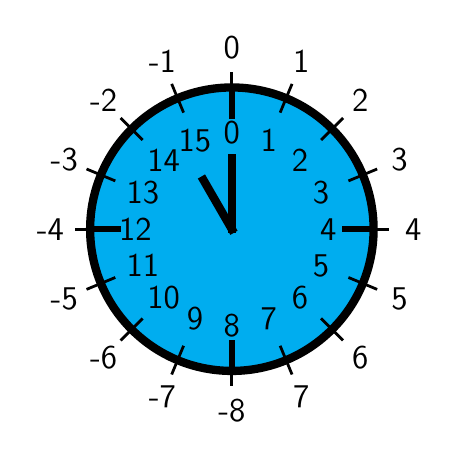
\begin{tikzpicture}[line cap=rect,line width=3pt,scale=0.9]
                    \filldraw [fill=cyan] (0,0) circle [radius=2cm];
                    \foreach \angle [count=\xi from 0] in {90,67.5,...,-247.5}
                    {
                        \draw[line width=1pt] (\angle:1.8cm) -- (\angle:2.2cm);
                        \node[font=\large] at (\angle:1.36cm) {\textsf{\xi}};
                    }
                    \foreach \angle [count=\xi from -8] in {270,247.5,...,-67.5}
                    {
                        \node[font=\large] at (\angle:2.56cm) {\textsf{\xi}};
                    }
                    \foreach \angle in {0,90,180,270}
                        \draw[line width=2pt] (\angle:1.6cm) -- (\angle:2cm);
                    \draw (0,0) -- (120:0.8cm);
                    \draw (0,0) -- (90:1cm);
                \end{tikzpicture}
            \end{center}
        \end{column}
        \begin{column}{0.55\textwidth}
            \begin{itemize}
                \pause\item Arithmetic \textbf{modulo} $N$
                \pause\item Numbers ``wrap around'' between $0$ and $N-1$
                \pause\item E.g.\ modulo $16$:
                    \begin{itemize}
                        \pause\item $14 + 7 = 5$
                        \pause\item $4 - 7 = 13$
                    \end{itemize}
            \end{itemize}
        \end{column}
    \end{columns}
\end{frame}

\begin{frame}{Modulo operator}
    \begin{itemize}
        \pause\item Present in many programming languages (including C++, C\#, Python) as \lstinline{\%}
        \pause\item \lstinline{a \% b} gives the \textbf{remainder} of \lstinline{a} divided by \lstinline{b}
        \pause\item E.g.\ \lstinline{21 \% 16} gives 5
        \pause\item Useful for wrapping around e.g.\ loop indexes or screen coordinates
    \end{itemize}
\end{frame}

\begin{frame}{2's complement}
    \begin{itemize}
        \pause\item How can we represent negative numbers in binary?
        \pause\item Represent them modulo $2^n$ (for $n$ bits)
        \pause\item I.e.\ represent $-a$ as $2^n-a$
        \pause\item Instead of an $n$-bit number ranging from $0$ to $2^n-1$, it ranges from $-2^{n-1}$ to $+2^{n-1}-1$
        \pause\item E.g.\ 16-bit number ranges from $-32768$ to $+32767$
        \pause\item Note that the left-most bit can be interpreted as a \textbf{sign} bit:
            $1$ if negative, $0$ if positive or zero
    \end{itemize}
\end{frame}

\begin{frame}{Converting to 2's complement}
    \begin{itemize}
        \pause\item Convert the absolute value to binary
        \pause\item Invert all the bits (i.e.\ change $0 \leftrightarrow 1$)
        \pause\item Add 1
        \pause\item (This is equivalent to subtracting the number from $2^n$... why?)
        \pause\item This is also the process for converting back from 2's complement,
            i.e.\ doing it twice should give the original number
    \end{itemize}
\end{frame}

\begin{frame}{Why 2's complement?}
    \begin{itemize}
        \pause\item Allows all addition and subtraction to be carried out modulo $2^n$
            without caring whether numbers are positive or negative
        \pause\item In fact, subtraction can just be done as addition
        \pause\item I.e.\ $a-b$ is the same as $a+(-b)$, where $a$ and $-b$ are just $n$-bit numbers
    \end{itemize}
\end{frame}

\part{Scientific notation}
\frame{\partpage}

\begin{frame}{Integer powers}
	Let $a \neq 0$ be a real number, and let $b > 0$ be an integer
	\pause
	$$ a^b = \underbrace{a \times a \times \dots \times a}_{\text{$b$ times}} $$
	\pause
	$$ a^0 = 1 $$
	\pause
	$$ a^{-b} = \underbrace{\frac{1}{a \times a \times \dots \times a}}_{\text{$b$ times}} $$
\end{frame}

\begin{frame}{Powers of 10}
	\pause
	$$ 10^6 = 1\underbrace{000\,000}_{\text{6 zeroes}} $$
	\pause
	$$ 10^1 = 10 $$
	\pause
	$$ 10^0 = 1 $$
	\pause
	$$ 10^{-1} = 0.1 $$
	\pause
	$$ 10^{-6} = 0.\underbrace{000\,00}_{\text{5 zeroes}}1 $$
\end{frame}

\begin{frame}{Multiplying by powers of 10}
	\pause
	Multiplying by $10^n$ is the same as moving the decimal point $n$ places to the \textbf{right}
	(adding zeroes if necessary)
	\pause
	$$ 3.14159 \times 10^2 = 314.159 $$
	\pause
	$$ 27 \times 10^3 = 27\,000 $$
	\pause
	Similarly if $n$ is negative, the decimal point moves to the \textbf{left}
	\pause
	$$ 123.45 \times 10^{-2} = 1.2345 $$
\end{frame}

\begin{frame}{Scientific notation}
	\begin{itemize}
		\pause\item A way of writing \textbf{very large} and \textbf{very small} numbers
		\pause\item $a \times 10^b$, where
			\begin{itemize}
				\pause\item $a$ ($1 \leq |a| < 10$) is the \textbf{mantissa}
				\pause\item ($a$ is a positive or negative number
					with a single non-zero digit before the decimal point)
				\pause\item $b$ (an integer) is the \textbf{exponent}
			\end{itemize}
		\pause\item E.g.\ 1 light year = $9.461 \times 10^{15}$ metres
		\pause\item E.g.\ Planck's constant = $6.626 \times 10^{-34}$ joules
		\pause\item Socrative \texttt{FALCOMPED}
	\end{itemize}
\end{frame}

\begin{frame}[fragile]{Scientific notation in code}
	\pause Instead of writing \fbox{$\times 10$}, write \fbox{\lstinline{e}} (no spaces)
	\pause
	\begin{lstlisting}
double lightYear = 9.461e15;
double plancksConstant = 6.626e-34;
	\end{lstlisting}
\end{frame}


\part{Floating point numbers}
\frame{\partpage}

\begin{frame}{Floating point numbers}
	\begin{itemize}
		\pause\item Similar to scientific notation, but \textbf{base 2} (binary)
		\pause\item $a \times 10^b$, where
			\begin{itemize}
				\pause\item $a$ ($1 \leq |a| < 2$) is the \textbf{mantissa}
				\pause\item ($a$ is a positive or negative number
					with a single $1$ before the ``decimal point'')
				\pause\item $b$ (an integer) is the \textbf{exponent}
			\end{itemize}
	\end{itemize}
\end{frame}

\begin{frame}{Storing the mantissa}
	\begin{itemize}
		\pause\item A positive or negative number with a single $1$ before the ``decimal point''
		\pause\item Sign is stored as a single bit: $0=+$, $1=-$
		\pause\item We know there's a $1$ before the point so no need to store it --- just store the binary
			digits after the point
	\end{itemize}
\end{frame}

\begin{frame}{Storing the exponent}
	\begin{itemize}
		\pause\item An integer --- can be positive, negative or zero
		\pause\item NB we don't use 2's complement to store it!
		\pause\item Instead it is stored in binary as a positive integer with a \textbf{bias} added on
		\pause\item (This is so that exponents can be efficiently compared (less/greater than)
			--- 2's complement would be less efficient for this)
	\end{itemize}
\end{frame}

\begin{frame}{Exponent bias}
	\begin{itemize}
		\pause\item E.g.\ if the bias is $127$:
	\end{itemize}
	\pause
	\begin{center}
		\begin{tabular}{|r|l|}
			\hline
			An exponent of... & ... is stored as \\\hline
			-126 & 00000001 (1) \\
			\vdots & \vdots \\
			-1 & 01111110 (126) \\
			0 & 01111111 (127) \\
			1 & 10000000 (128) \\
			\vdots & \vdots \\
			127 & 11111110 (254) \\\hline
		\end{tabular}
	\end{center}
	\begin{itemize}
		\pause\item (Exponents of 00000000 and 11111111 have special meaning --- more on this later)
	\end{itemize}
\end{frame}

\begin{frame}[fragile]{IEEE 754 floating point formats}
	\begin{center}
		\begin{tabular}{|r|ccc|l|}
			\hline
			Type & Sign & Exponent & Mantissa & Total \\\hline
			Single precision & 1 bit & 8 bits & 23 bits & 32 bits \\
			&& bias 127 && \\\hline
			Double precision & 1 bit & 11 bits & 52 bits & 64 bits \\
			&& bias 1023 && \\\hline
			Extended precision & 1 bit & 15 bits & 64 bits & 80 bits \\
			&& bias 16383 && \\\hline
		\end{tabular}
	\end{center}
\end{frame}

\begin{frame}[fragile]{IEEE 754 floating point formats}
	\begin{itemize}
		\pause\item C\# (and many other languages) have \lstinline{float} and \lstinline{double} types
			for single and double precision respectively
		\pause\item Literals are interpreted as \lstinline{float} if they end in \lstinline{f}, otherwise \lstinline{double}
			\begin{itemize}
				\pause\item \lstinline{3.14f} is a \lstinline{float}
				\pause\item \lstinline{3.14} is a \lstinline{double}
			\end{itemize}
		\pause\item Python's \lstinline{float} type is double precision as standard
		\pause\item Extended precision is not usually used in programs, but is used internally on Intel CPUs
	\end{itemize}
\end{frame}

\begin{frame}{Example}
	\pause
	What is the value stored in the following IEEE single-precision floating point number?
	\begin{center}
		\texttt{01000000110100000000000000000000}
	\end{center}
\end{frame}

\begin{frame}{Example}
	\pause
	\begin{center}
		\texttt{\fbox{0}1000000110100000000000000000000}
	\end{center}
	\begin{itemize}
		\pause\item Sign bit is 0
		\pause\item Therefore the number is positive
	\end{itemize}
\end{frame}

\begin{frame}{Example}
	\pause
	\begin{center}
		\texttt{0\fbox{10000001}10100000000000000000000}
	\end{center}
	\begin{itemize}
		\pause\item Exponent is 10000001
		\pause\item This is 129 in binary
		\pause\item Exponent is stored with a bias of 127, therefore the actual exponent is
			$129 - 127 = 2$
	\end{itemize}
\end{frame}

\begin{frame}{Example}
	\pause
	\begin{center}
		\texttt{010000001\fbox{10100000000000000000000}}
	\end{center}
	\begin{itemize}
		\pause\item Mantissa is $101000\dots$
		\pause\item Remember we only store the digits after the ``decimal point'', so the mantissa
			is actually $1.101000\dots$
		\pause\item The exponent is 2, so we move the point 2 places to the right:
			$110.1000\dots$
		\pause\item $4 + 2 + \frac12 = 6.5$
	\end{itemize}
\end{frame}

%\begin{frame}{Socrative \texttt{FALCOMPED}}
	%\pause
	%What is the value of this number expressed in IEEE 754 single precision format?
	%\begin{center}
		%\texttt{0 10000010 01011000000000000000000}
	%\end{center}
	%You have \textbf{5 minutes}, and you \textbf{may} use a calculator!
	%(Unless your calculator does IEEE 754 conversion...)
%\end{frame}
%
%\iftoggle{printable}{}{
%\begin{frame}{Example}
	%\pause
	%\begin{center}
		%\texttt{0 10000010 01011000000000000000000}
	%\end{center}
	%\begin{itemize}
		%\pause\item Exponent: $130 - 127 = 3$
		%\pause\item Mantissa: binary $1.01011$
		%\pause\item $1 + \frac14 + \frac{1}{16} + \frac{1}{32} = 1.34375$
		%\pause\item $1.34375 \times 2^3 = 10.75$
		%\pause\item Alternatively: $1.01011 \times 2^3 = 1010.11$
		%\pause\item $= 8 + 2 + \frac12 + \frac14 = 10.75$
	%\end{itemize}
%\end{frame}
%}

\begin{frame}[fragile]{Special floating point numbers}
	\begin{itemize}
		\pause\item Zero is represented by a mantissa and exponent of all 0s
		\pause\item An exponent of all 1s is used to represent infinity or NaN
			\begin{itemize}
				\pause\item \lstinline{float.PositiveInfinity} or \lstinline{double.PositiveInfinity}:
					a number which is greater than every other number
				\pause\item \lstinline{float.NegativeInfinity} or \lstinline{double.NegativeInfinity}:
					a number which is less than every other number
				\pause\item \lstinline{float.NaN} or \lstinline{double.NaN}:
					``Not A Number'' --- \lstinline{<}, \lstinline{>}, \lstinline{==}
					always return \lstinline{false}
			\end{itemize}
		\pause\item Can check for these with \lstinline{float.IsInfinity},
			\lstinline{double.IsNaN}, etc.
		\pause\item Infinities and NaNs sometimes arise from calculations (e.g.\ dividing by zero)
	\end{itemize}
\end{frame}

\part{Numerical precision}
\frame{\partpage}

\begin{frame}{Precision of floating point numbers}
	\begin{itemize}
		\pause\item Precision \textbf{varies} by \textbf{magnitude}
		\pause\item Numbers near 0 can be stored more accurately than numbers further from 0
		\pause\item Analogy: in scientific notation with 3 decimal places
			\begin{itemize}
				\pause\item Around $3.142 \times 10^0$: can represent a difference of $0.001$
				\pause\item Around $3.142 \times 10^3$: can represent a difference of $1$
				\pause\item Around $3.142 \times 10^6$: can represent a difference of $1000$
			\end{itemize}
	\end{itemize}
\end{frame}

\begin{frame}[fragile]{Range of floating point numbers}
	\begin{center}
		\begin{tabular}{|r|cc|}
			\hline
			Type & Smallest value & Largest value \\
			& (closest to 0) & (furthest from 0) \\\hline
			Single precision & $\pm 1.175 \times 10^{-38}$ & $\pm 3.403 \times 10^{38}$ \\\hline
			Double precision & $\pm 2.225 \times 10^{-308}$ & $\pm 1.798 \times 10^{308}$ \\\hline
		\end{tabular}
	\end{center}
\end{frame}

\begin{frame}{Rounding errors}
	\begin{itemize}
		\pause\item Many numbers cannot be represented exactly in IEEE float
			\begin{itemize}
				\pause\item Similar to how decimal notation cannot exactly represent
					$\frac13 = 0.3333333\dots$ or $\frac17 = 0.142857\dots$
			\end{itemize}
		\pause\item Decimal: can represent $\frac{a}{b}$ exactly iff $b = 2^m 5^n$
		\pause\item Binary: can represent $\frac{a}{b}$ exactly iff $b = 2^n$
		\pause\item In particular, IEEE float can't represent $\frac{1}{10} = 0.1$ exactly!
		\pause\item This can lead to \textbf{rounding errors} with some calculations
	\end{itemize}
\end{frame}

\begin{frame}[fragile]{Testing for equality}
	\begin{itemize}
		\pause\item Due to rounding errors, using \lstinline{==} or \lstinline{!=} with floating point numbers is almost always a bad idea
		\pause\item E.g.\ in most languages, \lstinline{0.1 + 0.2 == 0.3} evaluates to \lstinline{false}!
		\pause\item Better to check for \textbf{approximate equality}: calculate the difference between the numbers,
			and check that it's smaller than some threshold
		\pause\item E.g.\ Unity has \lstinline{Mathf.Approximately} which does exactly this
	\end{itemize}
\end{frame}

\begin{frame}[fragile]{Decimal type}
	\begin{itemize}
		\pause\item C\# has a \lstinline{decimal} type
		\pause\item Uses base 10 rather than base 2, so avoids some of the surprises of IEEE float
		\pause\item ... however not natively supported by the CPU, hence much slower than \lstinline{float}/\lstinline{double}
	\end{itemize}
\end{frame}
%\part{Vectors}
\frame{\partpage}

\begin{frame}{Vectors}
	\begin{columns}
		\begin{column}{0.48\textwidth}
			\pause A vector has \textbf{components}
			\pause 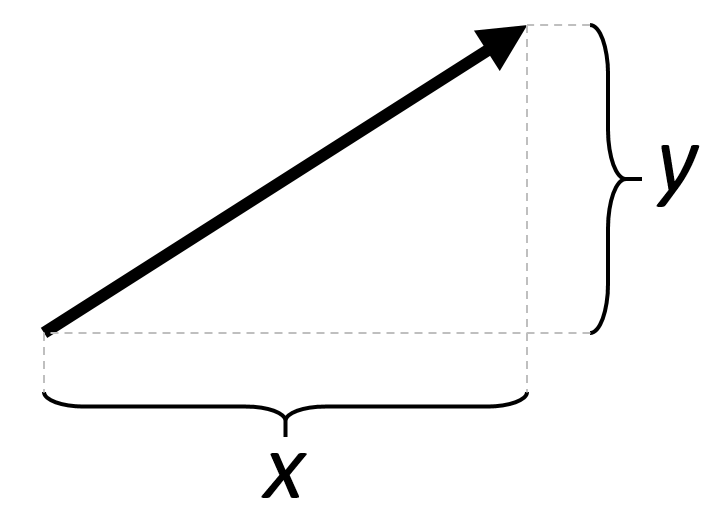
\includegraphics[width=\textwidth]{vector_components}
		\end{column}
		\begin{column}{0.48\textwidth}
			\pause A vector also has \textbf{direction} and \textbf{magnitude} (or \textbf{length})
			\pause 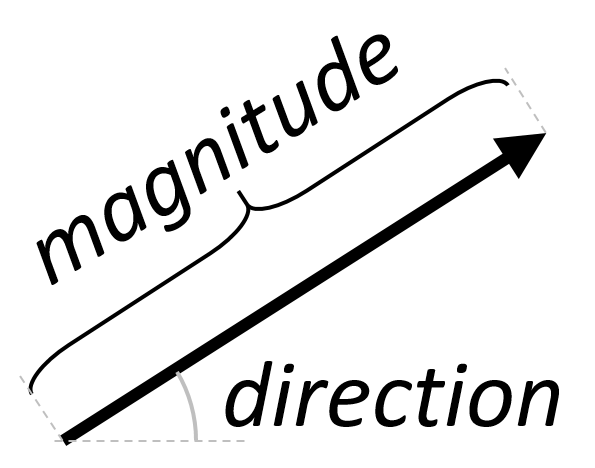
\includegraphics[width=\textwidth]{vector_polar}
		\end{column}
	\end{columns}
	\pause The \textbf{origin} is the point represented by the vector $(0, 0, \dots)$
\end{frame}

\begin{frame}{Radians}
	\begin{itemize}
		\pause\item We often measure angles in \textbf{radians}
		\pause\item $\pi = 3.14159\dots$ 
		\pause\item $\pi \text{ radians} = 180 \text{ degrees} = \text{half a circle}$ 
		\pause\item $\frac{\pi}{2} \text{ radians} = 90 \text{ degrees} = \text{right angle}$
		\pause\item Careful! Some things in OpenGL work in \textbf{degrees}, others in \textbf{radians}
			(just to confuse you...)
	\end{itemize}
\end{frame}

\begin{frame}{Right hand rule}
	\pause OpenGL uses a \textbf{right-handed coordinate system}
	\pause \begin{center}
		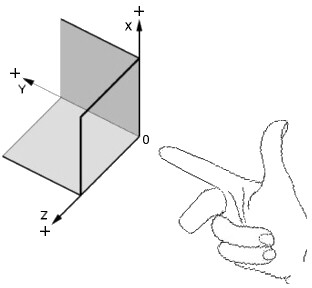
\includegraphics[width=0.3\textwidth]{RightHandRule}
	\end{center}
	\begin{itemize}
		\pause\item The \textbf{$x$-axis} points towards the \textbf{right-hand side} of the screen
		\pause\item The \textbf{$y$-axis} points towards the \textbf{top} of the screen
		\pause\item The \textbf{$z$-axis} points \textbf{out} of the screen
	\end{itemize}
\end{frame}

\begin{frame}{Homogeneous coordinates}
	\begin{itemize}
		\pause\item In 3D graphics, it is useful to represent a \textbf{point in 3D space} as a \textbf{4-dimensional vector}
		\pause\item The extra coordinate is called $w$
		\pause\item Simple explanation: $w$ should always equal $1$ for points in 3D space; having $w$ there makes certain calculations easier
			\begin{itemize}
				\pause\item (Actually, a point $(x,y,z)$ can be represented as a vector $(x \times w, y \times w, z \times w, w)$ for any $w \neq 0$)
			\end{itemize}
		\pause\item In homogeneous coordinates, the origin is $(0, 0, 0, 1)$ not $(0, 0, 0, 0)$!
	\end{itemize}
\end{frame}


\end{document}
